\chapter{Intégration}
\section{Intégrale et aire}
\subsection{Cas d'une fonction positive sur un intervalle donné.}

\begin{definition}[Intégrale]
    Soit \(f \in C^{0}(\left[ a;b \right], \mathbb{R}^{+})\) de courbe représentative \(\mathcal{C}_{f}\) dans un repère \((O,\vec{i},\vec{j})\) du plan. \par
    On appelle intégrale de \(a\) à \(b\) de la fonction \(f\) notée \( \int_{a}^{b} dx \,\)l'aire du domaine délimité par \(\mathcal{C}_{f}\), \((Ox)\) et les droites déquation \(x=a\), \(x=b\).

\end{definition}

\begin{figure}[!htb]
\centering
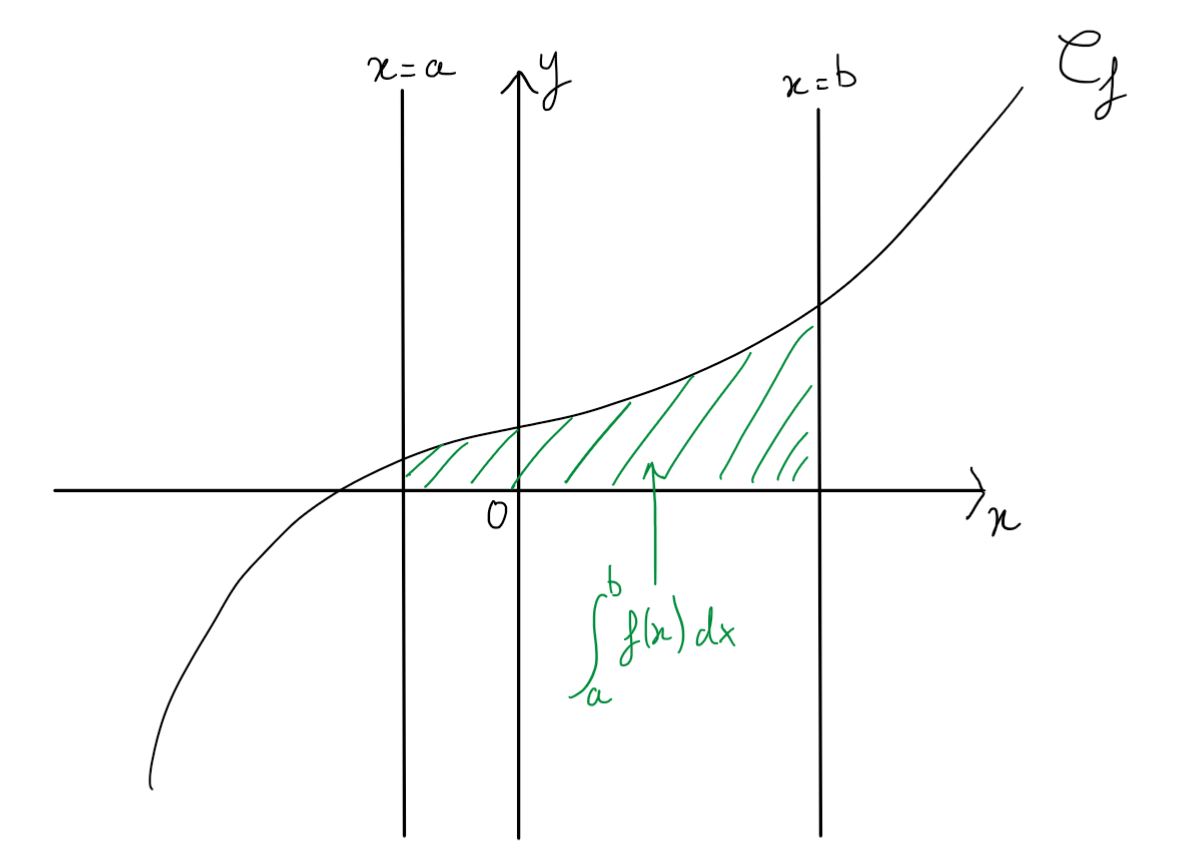
\includegraphics[width=0.5\textwidth]{SCHEMA-1.png}
\caption{Défintion de l'intégrale}
\label{fig:SCHEMA-1}
\end{figure}


\begin{remark}[Unités]
    L'aire du domaine est exprimée en unités d'aire (\(u.a\)) égale à l'aire du parallelogramme engendré par \(\vec{i}\) et \(\vec{j}\).\par
    \begin{itemize}
        \item Si le repère est orthogonal, le parallelogramme est un rectangle. 
        \item Si le repère est orthonormé, le parallelogramme est un carré.
    \end{itemize}
\end{remark}

\begin{eg}[Exemples]\par
    %2SCHEMAS
    \(I_{1} = \int_{0}^{1} x dx \,\)On reconnait un triangle rectangle de base 1 et de hauteur 1. \(I_{1} = \frac{1 \times 1}{2} = \frac{1}{2}\). \par
    \(I_{2} = \int_{1}^{2} 2x+1 dx \,\)On reconnait un parallelogramme rectangle. \(I_{2} = \frac{(3+5)1}{2} = 4\)    
\end{eg}

\begin{remark}[Variable muette]
    La variable d'intégration est muette : 
    \[
        \int_{b}^{a} f(x) dx \, = \int_{b}^{a} f(u) du =  \int_{b}^{a} f(t) dt \dots  
    \]
\end{remark}

\begin{corollary}[Propriétés]\label{pdef}
    Soit \(f,g \in C^{0}([a;b],\mathbb{R}^{+})\), soit \(c \in [a;b]\), soit \(\lambda \in \mathbb{R}\) 

    \begin{corollary}[Relation de Chasles]
        \[
            \int_{a}^{b} f(x) dx \, = \int_{a}^{c} f(x) dx \, \int_{c}^{b} f(x) dx. 
        \]  
    \end{corollary}

    \begin{corollary}[Valeur moyenne]
        La valeur moyenne \(\mu\) de \(f\) entre \(a\) et \(b\) est la valeur tel que l'integrale de f est égale au rectangle de hauteur \(\mu \).
        \[
            \mu = \frac{1}{b-a} \int_{b}^{a} f(x) dx
        \]  
    \end{corollary}

    \begin{corollary}[Linéarité et Ordre].  \par
        \begin{itemize}
            \item \( \int_{a}^{b} \lambda f(x) + g(x) dx = \lambda \int_{a}^{b} f(x) dx + \int_{a}^{b} g(x) dx\) 
            \item \(\forall x \in [a,b], f(x) \leq g(x) \implies \int_{a}^{b} f(x) dx \leq \int_{a}^{b} g(x) dx\) 
        \end{itemize}
        Pour l'ordre, il n'y a pas d'équivalence.
    \end{corollary}
\end{corollary}

\begin{figure}[!htb]
    \centering
    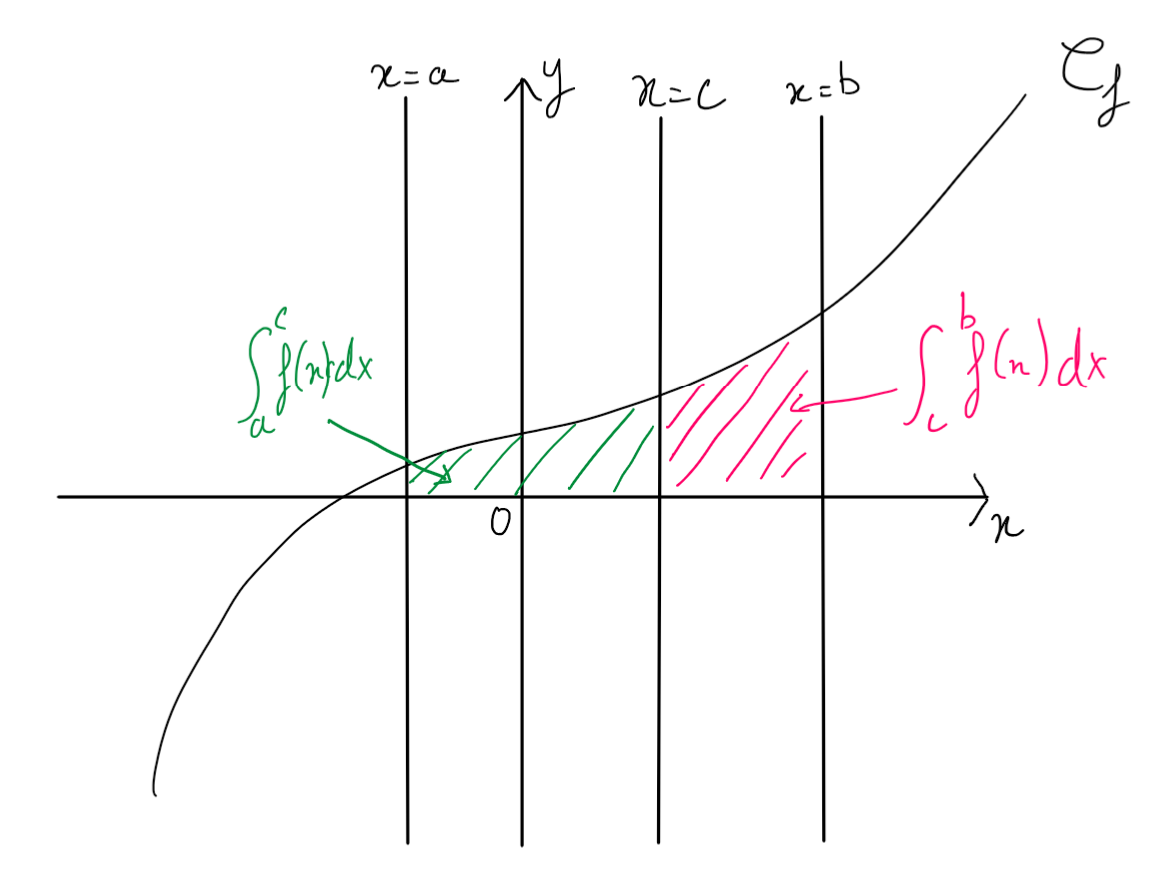
\includegraphics[width=0.4\textwidth]{SCHEMA-2.png}
    \caption{La relation de Chasles}
    \label{fig:SCHEMA-2}
\end{figure}

\begin{figure}[!htb]
    \centering
    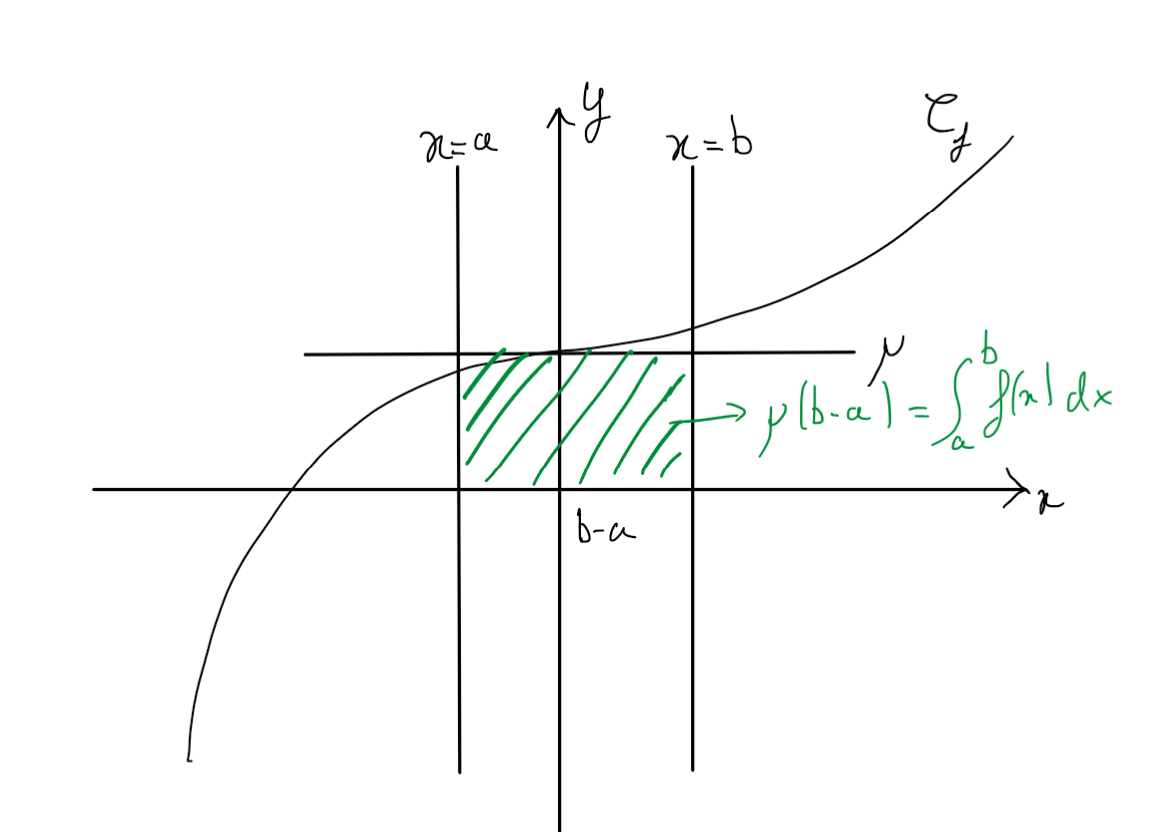
\includegraphics[width=0.4\textwidth]{SCHEMA-3.png}
    \caption{\(\mu\), la valeur moyenne d'une fonction }
    \label{fig:SCHEMA-3}
\end{figure}

\newpage
\subsection{Cas d'une fonction négative sur un intervalle donné}

\begin{definition}[Intégrale d'une fonction négative]
    Soit \(f \in C^{0}([a;b], \mathbb{R}^{-})\). \par
    L'intégrale de \(f\) entre \(a\) et \(b\) est l'opposé de l'aire géométrique du domaine délimité par, \(\mathcal{C}_f\), \((Ox)\), \(x=a\) et \(x=b\). C'est donc une aire algébrique et non géométrique.    
\end{definition}
\begin{figure}[!htb]
    \centering
    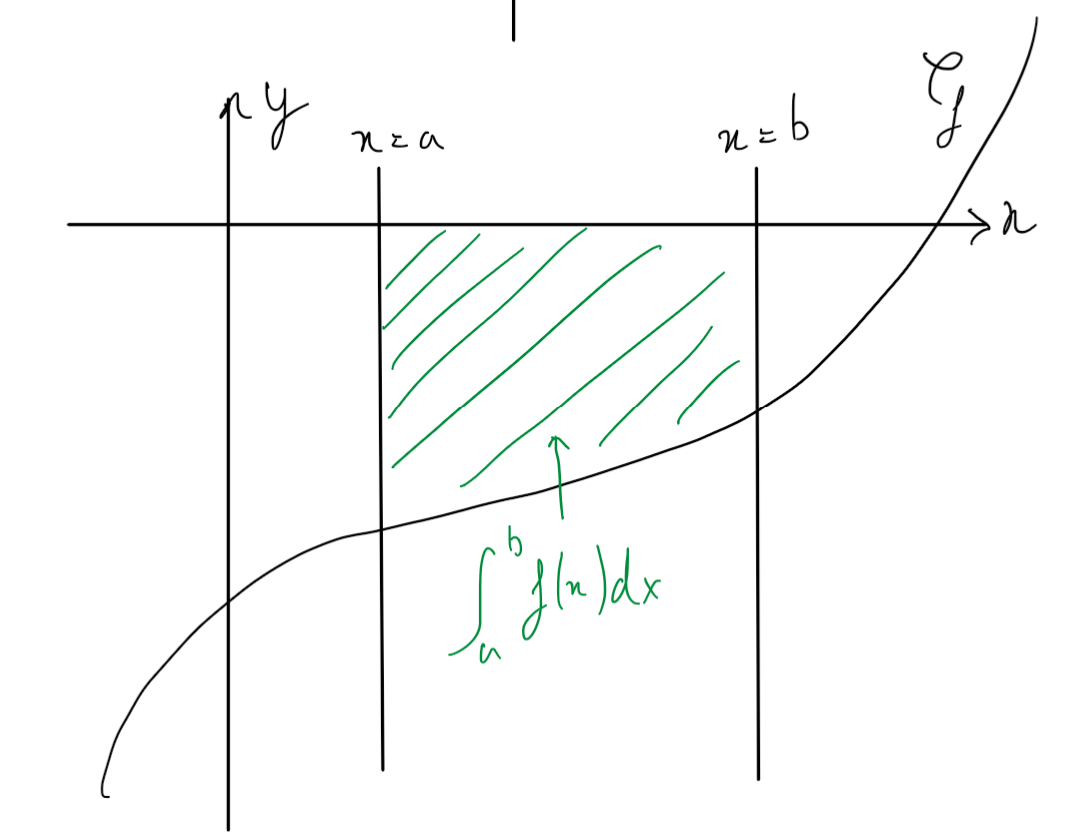
\includegraphics[width=0.5\textwidth]{SCHEMA-4.png}
    \caption{Intégrale d'une fonction négative}
    \label{fig:SCHEMA-4}
\end{figure}

\begin{corollary}[Propriétés]
    Les propriétés sont les mêmes que pour les fonctions négatives, voir \autoref{pdef}. 
\end{corollary}

\subsection{Cas d'une fonction de signe quelconque}

\begin{figure}[!htb]
    \centering
    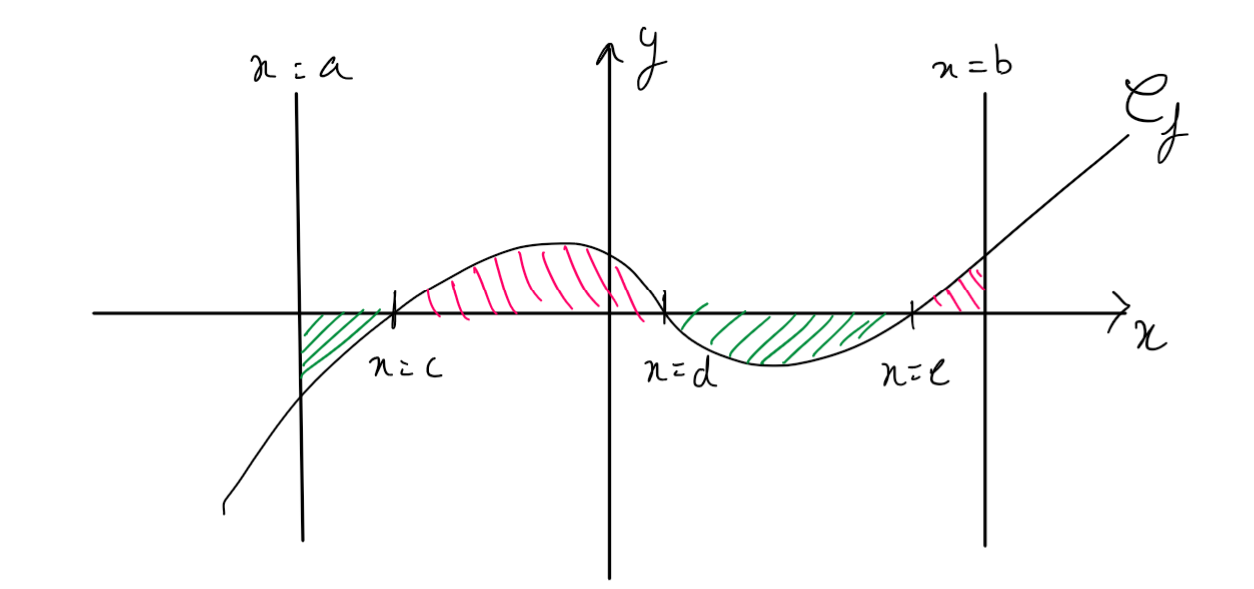
\includegraphics[width=0.5\textwidth]{SCHEMA-5.png}
    \caption{Décomposition d'une fonction sur des intervalles ou le signe est monotne}
    \label{fig:SCHEMA-5}
\end{figure}


\begin{definition}[Integrale d'une fonction de signe quelconque]
    Soit \(f \in C^{0}([a;b],\mathbb{R})\), pour définir l'intégrale de \(f\) entre \(a\) et \(b\) on utilise Chasles pour décomposer f sur des intervalles où \(f\) est de signe constant : 
    \[
        \int_{a}^{b} f dx = \int_{a}^{c} f dx + \int_{c}^{d} f dx + \int_{d}^{e} f dx + \int_{e}^{b} f dx
    \] 
\end{definition}

\begin{corollary}[Propriétés]
    On a les mêmes propriétés que sur les fonctions de signe constant (voir \autoref{pdef}). \par
    \begin{corollary}[Simplification]
        \begin{eqnarray*}
            \int_{a}^{a} f(x) dx &=& 0 \\
            \int_{a}^{b} f(x) dx &=& - \int_{b}^{a} f(x) dx
        \end{eqnarray*}
    \end{corollary}
    \begin{explanation}
        \[
            0 = \int_{a}^{a} f(x) dx = \int_{a}^{b} f(x) dx + \int_{b}^{a} f(x) dx \implies \int_{a}^{b} f(x) dx  = - \int_{b}^{a} f(x) dx \,\square
        \]
    \end{explanation}
    \begin{corollary}[Fonctions périodiques]
        Soit \(f \in C^{0}(\mathbb{R},\mathbb{R}), \text{ t.q. } f(x+T) = f(x)\), soit \(\lambda \in \mathbb{R}\) \par
        \[
            \int_{a}^{b} f(x) dx = \int_{a+\lambda T}^{b+\lambda T}  f(x) dx
        \]
    \end{corollary}
    \begin{corollary}[Fonctions paires]
        Soit \(f \in C^{0}, f(x) = f(-x)\).
        \[
            \int_{a}^{b} f(x) dx = \int_{-b}^{-a} f(x) dx \implies \int_{-a}^{a} f(x) dx = 2 \int_{0}^{a} f(x) dx
        \] 
    \end{corollary}

    \begin{corollary}[Fonctions impaires]
        Soit \(f \in C^{0} \text{ t.q. } f(x) = -f(-x)\)
        \[
            \int_{-a}^{a} f(x) dx = 0
        \] 
    \end{corollary}
    \begin{corollary}[Fonctions bornées]
        Soit \(f \in C^{0} \implies \exists (M;m) \in \mathbb{R}^{2}, \forall x \in [a;b] m \leq f(x) \leq M\). 
        \begin{eqnarray*}
            &\implies& m \leq \mu \leq M \\
            &\implies& (b-a)m \leq \int_{a}^{b} f(x) dx \leq (b-a)M
        \end{eqnarray*}
    \end{corollary}
\end{corollary}

\begin{remark}[Intégrale d'une fonction constante] Soit \(k \in \mathbb{R}\) 
    \[
        \int_{a}^{b} k dx = k(b-a)
    \]
\end{remark}

\section{Primitive d'une fonction}

\begin{theorem}[Théorème fondamentale de l'analyse]
    \[
        \int_{a}^{b} f'(x) dx = f(b) - f(a)
    \]
\end{theorem}